\chapter{Materials and methods} \label{material_methods}

\section{Research area} \label{research_area}
The Canton of Zug was chosen by the author - who was raised in Cham - as the area of interest since important local knowledge was already present. The specific areas for which social media data (SMD) was acquired are visible in the map below (see figure \ref{fig:research_area}). The turquoise area resembles the political border of the Canton of Zug for which SMD for the social media platforms (SMP) Flickr and Foursquare were collected. The purple area is included in the above mentioned perimeter of the Canton of Zug and consists of three major areas. In the North lies the 'Lorzenebene' (plane of the river Lorze). This area is of special interest to the cantonal authorities due to its local recreation value. An overall concept - named 'Leitbild Lorzenebene' has been created for it which was used as reference in this thesis \cite{BaudirektiondesKantonsZug2012LeitbildBericht}. The second area resembles the jurisdiction of the City of Zug which partly encompasses the 'Lorzenebene'. This area is distinctive by its internal urban gradient which increases towards the city centre as well as the long reaching lake side. The last area furthest South consists of the three mountains 'Zuger-, Walchwiler-, Rossberg' which are likewise part of an development concept \cite{Berchtold2011EntwicklungsleitbildRossberg} of the Canton of Zug due to their sport and recreation value. \\
There is no perimeter concordance due to varying constraints in the data acquisition between the different social media platforms which will be illustrated further down in section \ref{data_acquisition}.

\begin{figure}[h]
   \centering
   \includegraphics[width=0.75\textwidth]{img/overview_research_area_w_Lorzenebene.eps}
   \caption{Overview over the data acquisition perimeters}
   \label{fig:research_area}
\end{figure}


\section{Data acquisition and composition} \label{data_acquisition}
The following subsections will elaborate on the data-acquisition process and the data-composition of the three SMP used in this thesis. 

\subsection{Instagram} \label{instagram}
Instagram is a SMP which supports the sharing of geo-referenced image and video content. The platform is mostly financed by web-advertisement and belongs to \textit{Facebook Inc.} It can be accessed via the URL \texttt{https://www.instagram.com/} or the corresponding mobile application.
Instagram held roughly 2'529'000 users in Switzerland on January 2019 which accounted for 29.4\% of its population. People aged 25 to 34 were the largest user group (780' 000). The gender distribution was at 49.4\% women and 50.6\% men \cite{NapoleonCat2019NoTitle}. This popularity was the determining factor that lead to including Instagram data into this thesis.\\

\subsubsection{Query} \label{netlytic}
Licensed Instagram data of the research area visible in figure \ref{fig:research_area} has been collected via the cloud-based text and social media analyser \textit{Netlytic}. \textit{Netlytic} can be accessed via \texttt{https://netlytic.org/} and allows for hashtag (\# + keyword) or location driven queries. Former allows to search for Instagram media objects by providing decisive keywords which are preceded by a '\#'. The latter was used in the scope of this thesis which allows location based query for Instagram media objects of public accounts in a 5km radius around a given point. The used \textit{Netlytic} query points with their given perimeter are visible in figure \ref{fig:research_area}. The exact latitude / longitude coordinate pairs are the following:\\
\begin{enumerate}
  \item 47.177068, 8.494803
  \item 47.129913, 8.533604
  \item 47.104457, 8.570291
\end{enumerate}

\subsubsection{Time-span} \label{Instagram_timespan}
Data collection has been continuously performed over all three queries from the 30.09.2018 till the 11.12.2018. Due to the retirement of the Instagram Application Program Interface (API) on the 11.12.2018 \cite{Instagram2018InstagramRetirement} this period could not be extended.

\subsubsection{Data} \label{Instagram_data}
The data-collection accounted for 28'246 raw Instagram media objects. After the dominant authors and bulk-upload data-processing steps referenced further down (see chapter (\ref{data_processing}) 11'777 remained.
The data provided by \textit{Netlytic} came in the Comma Separated Values (CSV) format. Every media object was provided with the following information entities with the appropriate PostgreSQL data type in square brackets:
\begin{itemize}
    \item id : Unique media object identifier. [varchar(30)] if the media object contains location information, [numeric(20)] if not.
    \item latitude and longitude : Coordinate information in the WGS84 reference system of a specific Instagram location [double precision]
    \item link : URL to the actual media object on \texttt{https://www.Instagram.com/} [text]
    \item media-link : URL directing solely to the image content [text]
    \item publication date : Date and time when the media object was uploaded with the data-format YYYY-MM-DD HH:MM:SS [timestamp]
    \item author : The Instagram username of the media object author [text]
    \item title : User generated media object title [text]
    \item description : User generated media object description [text] 
    \item like-count : Amount of likes the media object received on the SMP Instagram
\end{itemize}

\paragraph{Location tag}
The provided location information or tag consists of the above mentioned coordinates of a Instagram location. Instagram locations are points of interest which can be user-generated and do not represent the actual precise coordinates where the media object was created. This has been implemented by Facebook as a further step to preserve the Instagram users anonymity by mitigating the divulging of sensitive location data. This implies that media objects that do not originate from the same location can still be 'snapped' to the same Instagram location and therefore show the same coordinate pair in the meta-data \cite{InstagramTags}.
It has been shown that roughly 85\% of Instagram media objects lack a location tag \cite{2018InstagramTags} and most users only use them on vacation or when being abroad.
Additional location related information (address) was gathered for all the media objects via the official Instagram API. More information can be found in chapter \ref{sec: XXXXX}


\subsection{Flickr} \label{flickr}
Flickr is photo sharing website (\texttt{https://www.flickr.com/}) that allows users to upload geo-reverenced images similar to Instagram. The corresponding free of charge Flickr API gives access to the entire database of Flickr media objects since the launch of the platform in the year 2005. The popularity of Flickr according to the 'Alexa Global Rank' lies at 349 \cite{Alexa.com2019AlexaFlickr} which is significantly lower than to the one of Instagram which lies at 16 \cite{Alexa.com2019AlexaInstagram}. Flickr still plays an important role also as data foundation for scientific studies due to the simple and unbounded data-access. <ADD REFERENCES>
DEMOGRPAHIC INFORMATION
WHY WAS IT CHOSEN
\subsubsection{Query} \label{flickr_query}
The entire Flickr database was queried via the publicly accessible official Flickr API. Media objects with a geo-reference-accuracy level of 12 or higher (maximum of 16) were of interest which resolves to city level up to street level. Queries were conducted by inputting several different bounding boxes which together cover the entire perimeter of the legal boundaries of the canton of Zug. Each bounding box was defined by two coordinate pairs, describing the bottom left and top right corner of a rectangle. This process of subdividing the area was necessary due to a maximum return threshold of 4'000 media objects per request. Therefore, to ensure the acquisition of the entire available data-set each bounding box had to hold less than 4'000 media objects.
\subsubsection{Time-span} \label{flickr_timespan}
The all the individual bounding-box API requests described above were queried for the time-spawn 2005 (launch of the SMP Flickr) until the 23rd of November 2018. 
\subsubsection{Data} \label{flickr_data}
The data that was returned by the Flickr API was in the JavaScript Object Notation (JSON) format. The following information has been extracted for every Flickr media object with the appropriate PostgreSQL data types in square brackets:\\

\begin{itemize}
    \item id : Unique media object identifier [bigint]
    \item latitude and longitude : Coordinate information in the WGS84 reference system [double precision]
    \item link : URL to the actual media object in the format \texttt{https://www.flickr.com/photos/[author]/[ID]/} [text]
    \item date taken : Time-stamp from the image meta-data stating when it was taken. 
    \item publication date : Time-stamp when the media object was uploaded to Flickr with the data-format MM/DD/YYYY HH:MM:SS [time-stamp]
    \item author : The Flickr username of the media object author [text]
    \item author id : Unique author identifier [text] 
    \item author origin : User given geographical information regarding the authors origin [text]
    \item title : User generated media object title [text]
    \item description : User generated media object description [text]
    \item tags : Keywords similar to Instagram hashtags that describe the media object but which are extracted by an image recognition algorithm similar to Google Cloud Vision \cite{Flickr2019FlickrRecognition}. (therefore already includes smart image labels!) [text]
    \item views : Amount of media object calls [bigint]
    \item favorites : Amount of approves - similar to 'likes' on Instagram - a media object received by other Flickr users [bigint]
\end{itemize}

\paragraph{Location tag}
Unlike Instagram provides Flickr location information or tags that represent the actual geographical position where the provided image was taken. This geotag is extracted from the meta-data of the image itself and can come in different accuracies ranging from 0 (global scale) to 16 (street level) dependant on the users preference or the GPS signal strength. \\
Additional location related information (address and location type) was gathered for all the media objects via the Google Geocoding API. More information can be found in chapter \ref{sec: XXXXX}

\subsection{Foursquare} \label{foursquare}
Foursquare is a platform which enables users to rate and share their visits and experiences to certain establishments (referred to as venues). All the stored ' infrastructure' which is categorised into different sectors such as ' Travel & Transport', ' Arts and Entertainment' but also ' Outdoors & Recreation' can be accessed via the official Foursquare API.
DEMOGRAPHIC INFORMATION
WHY WAS IT CHOSEN
\subsubsection{Query} \label{foursquare_query}
The following two API endpoints which return different information were used for this thesis.
\paragraph{Venue search (regular endpoint)} \label{foursquare_endpoint1}
The first step of the information acquirement involved a spatial search for venue ids of the category 'Outdoors & Recreation' that lie within the research area boundaries. This request was done with the regular venue search API endpoint. There was a limitation to the maximum number of results per request, similar to the bounding box request of Flickr. Therefore, a similar spatial subdivision of the research areas was used to query all the available venues, so that each individual request returned less than 50 results.
\paragraph{Acquiring venue details (premium endpoint)} \label{foursquare_endpoint2}
To obtain more specific information about each venue, a second (premium) Foursquare API endpoint was used. This venue details endpoint only allowed 50 requests per day for regular users which spread the data acquisition over 9 days. Insight among others on a more concrete subcategory description, the formatted address, the user rating as well as if the venue was verified or not was the result.

\subsubsection{Data} \label{fq_data}
The data returned by the Foursqure API and the above mentioned endpoints was in the JSON format - the same as the Flickr data.
Only the following excerpt of the returned venue meta-data was used with the appropriate PostgreSQL data types in square brackets: \\
\begin{itemize}
    \item venue id : Unique venue identifier [text]
    \item venue name : Locally used name to address the venue [text]
    \item latitude and longitude : Coordinate information in the WGS84 reference system [double precision]
    \item country name : Name of the country the venue is located in - used as additional data-verification [text]
    \item rating : Venue rating generated through Foursquare users [real]
    \item category id : Unique Foursquare venue category identifier [text]
    \item category name : Foursquare venue category name
    \item verified : Takes the values TRUE or FALSE. States if the venue data is verified by Foursquare
\end{itemize}

Additional location related information (address and location type) was gathered for all the media objects via the Google Geocoding API. More information can be found in chapter \ref{sec: XXXXX}

\subsubsection{Data verification} \label{foursquare_data_verification}
The data verification on Foursquare is not an automated process. It is done by manual supervision of Foursquare personnel. If a business can claim their venue which will initiate the Foursquare verification process. This processing is linked to a fee of roughly 20 USD for venues outside of the United States of America \cite{Foursquare2019FoursquareClaim}. \\
Of all 405 venues located inside the canton of Zug, 13 (3.2\%) are verified according to the data provided by the foursquare API. The remaining non-verified venues of the categories: scenic outlook, playground, athletics & sport, farm, (nudist) beach, lake, trail, golf course, mountain, campground, bathing area, outdoors & recreation, harbour, recreation centre, dog run, forest, pedestrian plaza, waterfront, basketball court, river, bike trail and skate park were evaluated by the author - who grew up in the area - to its best knowledge. XY venues belonged to said categories of which XY were verified by the author of this thesis.

\section{Database Setup} \label{database_setup}
During the course of this thesis a PostgreSQL database (\texttt{https://www.postgresql.org/}) was used which functioned as a centralised place to store the Flickr, Instagram and Foursquare data related to this project. The advantage of this approach compared to reading and storing in common txt- or csv-files is the possibility of computational efficient data-retrieval as by indexing conditional columns and data-manipulation through SQL queries. SQL is a standalone language for relational database management systems (RDBMS) which allows among other, smart table joins through primary and foreign key relation and conditional statements for advanced filtering \cite{PostgreSQL2019PostgreSQLDocumentation}.\\
Additionally, a Graphical User Interface (GUI) named pgAdmin4 (\texttt{https://www.pgadmin.org/}) - which is compatible with PostgreSQL - was used for the manually performed training-data verification process that is described in chapter \ref{XY}.\\
The following tables were created for the housing of the used data in this format: [object-type]\_[data-origin]\_[data-source] \\
\newline

Media object tables:\\
\begin{itemize}
    \item media\_objects\_cantonzug\_flickr
    \item media\_objects\_unionzug\_instagram
    \item media\_objects\_trainingdata\_instagram
    \item media\_objects\_cantonzug\_foursquare
\end{itemize}
\newline
Location tables:\\
\begin{itemize}
    \item locations\_cantonzug\_flickr
    \item locations\_unionzug\_instagram
\end{itemize}

In more detail, the media object tables store all data related to an object retrieved from one of the three SMP as stated in the corresponding subchapters above. Furthermore are the outputs from the data- and text-processing steps (see chapter \ref{XY}) stored in the database.\\ 
The Instagram and Flickr media object tables are linked via a primary key to the corresponding locations table, where unique media object location information is separately stored to reduce redundancy. This information exceeds the basic coordinates provided by the Flickr API and the stand-alone user generated location provided by Netlytic (Instagram) by acquiring additional geographic information via Googles Geocoding API and the Instagram API respectively (see chapter \ref{XXXX}). Time-stamps were normalised across all SMP to the YYYY-MM-DD HH-MM-SS format \\
\newline
The exact structure and table specific content of the database is visible in figure \ref{fig:database}

\begin{figure}[h]
   \centering
   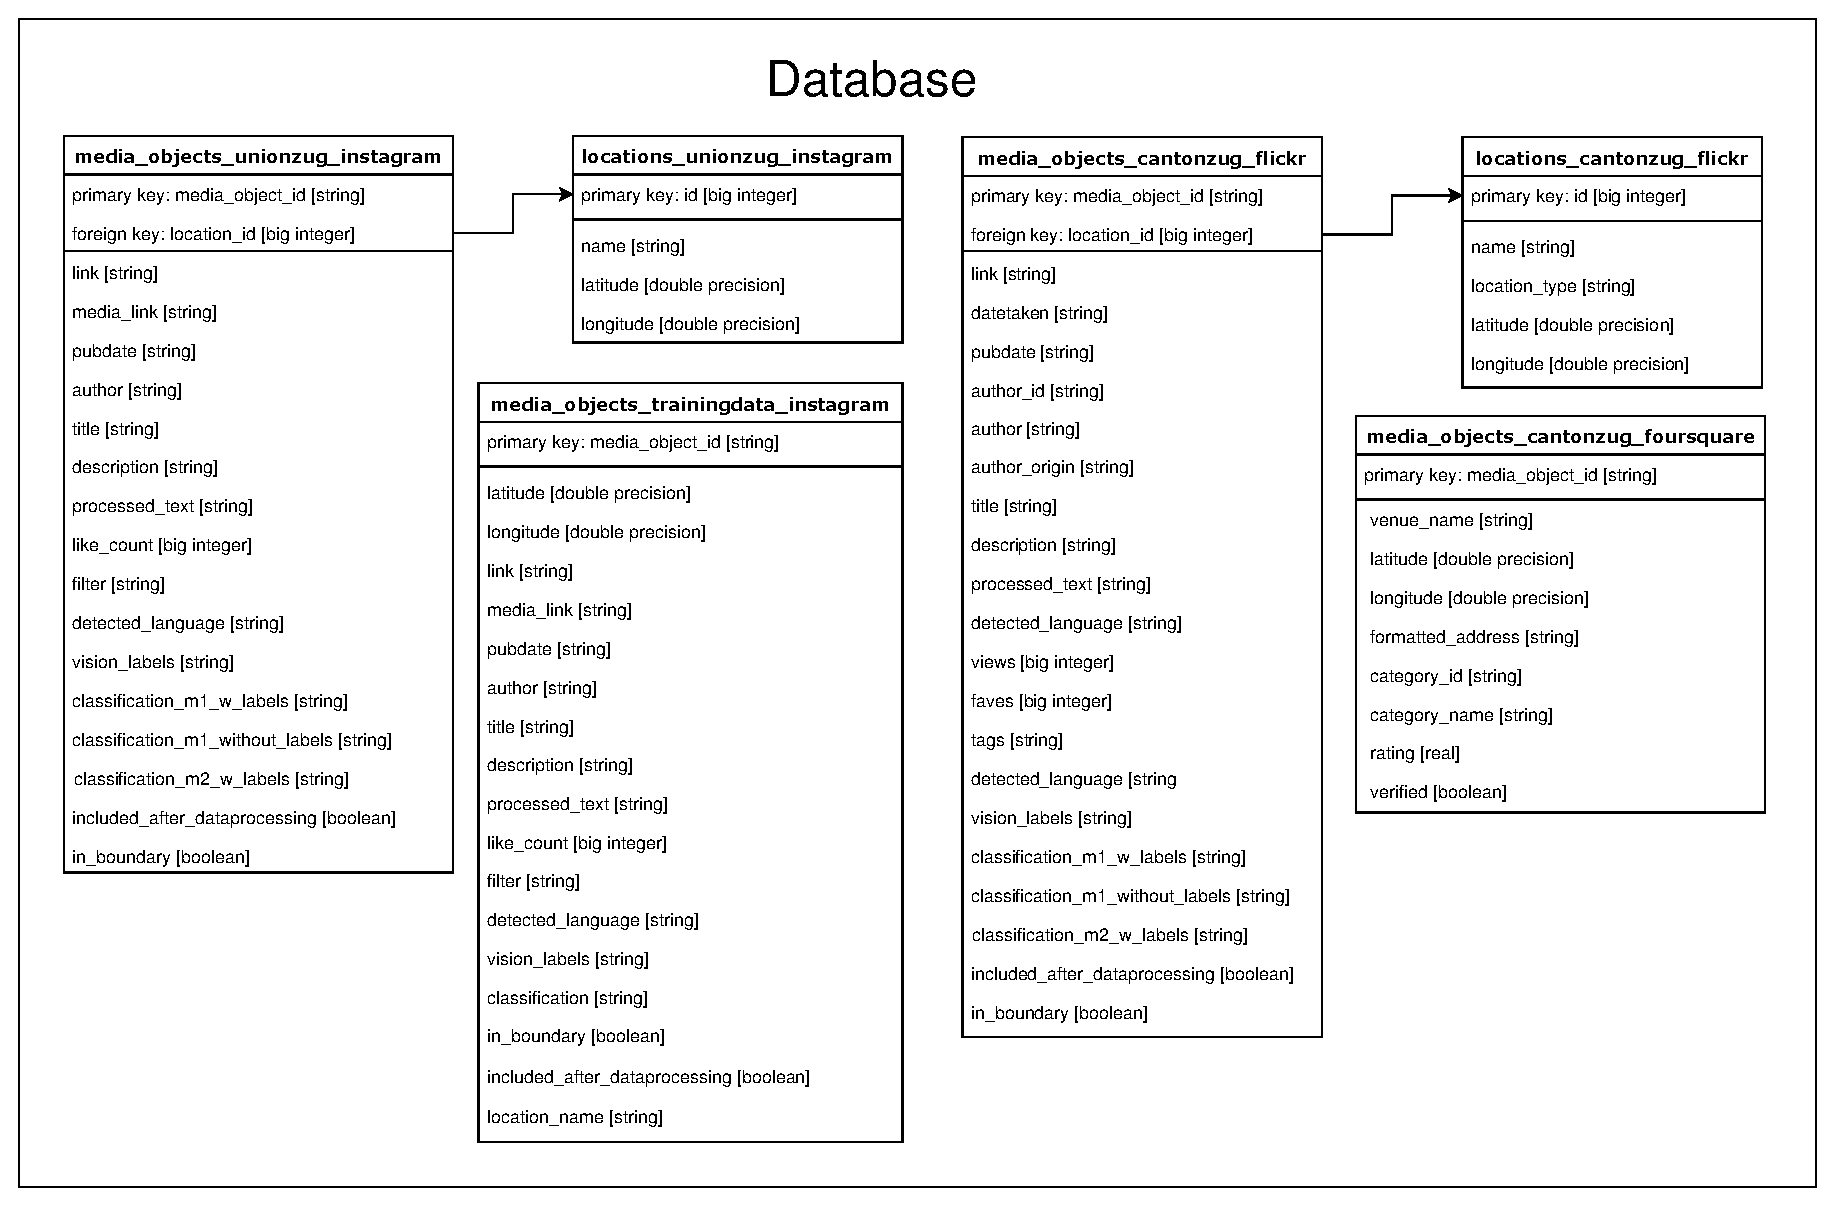
\includegraphics[width=0.75\textwidth]{img/fusion_db_overview.eps}
   \caption{Visualisation of the database, its associated tables and columns}
   \label{fig:database}
\end{figure}

\section{Data-processing} \label{data_processing}
The following processes cover the entire workflow of data manipulation on the database in the order they were executed.
\subsection{Merging of Instagram files} \label{netlytic_files_merge}
In total, three different, partly spatially overlapping Instagram queries were run via Netlytic. All of them returned one CSV file. they were merged to reduce the complexity of handling multiple files for the consecutive processes. Media object duplicates were also addressed in this step. This entire data-processing step was not needed for the Flickr-data since merging and duplicates were already handled during the data-mining.

\subsection{Acquisition of additional location information} \label{add_location_data}
Auxiliary, more detailed location information regarding the spatial origin of the media objects in the database were acquired. The following two subchapters will elaborate on this process for the different data sources Instagram and Flickr.

\subsubsection{Via the Instagram API}
The Instagram data that was provided by Netlytic was enhanced by using the \texttt{GET/locations/location-id} endpoint of the official Instagram API. Newly acquired information encompassed the Instagram location-name.

\subsubsection{Via the Google Geocoding API}
Each coordinate of every Flickr media object was run through the Google Geocoding API. Detailed information regarding the media objects address and location type was returned. The location type attribute is evidence of the API' s accuracy. Everything besides 'ROOFTOP' returns an address that is close but not exactly at the given coordinate and therefore an approximation.\\
The API has been called by modifying the following HTTPS-request:\\
\texttt{https://maps.googleapis.com/maps/api/geocode/json?latlng=[latitude,longitude]&key=[API\_KEY]}

\subsection{Populating the database} \label{populate_db}
The merged Instagram CSV-files and the Flickr CSV-files which were extended by the additional location information described in the subchapters above were used to populate the initial PostgreSQL database. This process was entirely done through the Python script provided in the Appendix \ref{XY} and the needed \textit{psycopg 2} library that functioned as linkage.

\subsection{Check the ' in boundary' condition} \label{in_boundary}
Additional area beyond the actual research area perimeters were queried due to the circular (Netlytic) or rectangular (Flickr API) shape of the spatial query perimeters. As consequence each acquired media object had to be checked to be inside the actual perimeter boundary. This process was accomplished with the open source Geographical Information Software (GIS) QGIS. The point data of all media objects was clipped to the appropriate research area and exported to a new CSV file. This CSV file was read by the Python script which updated the 'in\_boundary' column in the corresponding database entries to TRUE for the provided media objects.

\subsection{Potential sources of bias in the data} \label{sources_data_bias}
This part of the data-processing is a filtering step as seen in step 1 of figure \ref{XY} to eliminate media objects which would distort the \textbf{general} perception of the research question at hand: When and where are people performing NBRAs?

\subsubsection{Dominant authors} \label{bias_dominant_authors}
Authors (person who contributes to a given social media platform by uploading media objects) which are above a certain threshold regarding their total number of uploaded media objects in the research area, are marked in the database table column 'included\_after\_dataprocessing' as \texttt{False} and are thereby excluded from further analysis. There is a need to address dominant authors, because otherwise the data evaluation will be unequally based on a small number of users that contributed a lot to the entire data-set.\\
\newline
\textbf{How was this threshold defined?}\\
\newline
Two possibilities were considered:
\begin{enumerate}
  \item A static, top percentage of authors will be excluded
  \item A fixed amount of the most contributing authors will be excluded
\end{enumerate}

At first, a top 0.1\% threshold was implemented. Later in the development of the thesis a 'posts per author' distribution graph was simultaneously created as soon as the data was read into the database. The user is able to adapt the graph by inputting a desired number of top authors which should be included in the graph. This enables a data specific dynamic adaption of the threshold according to the user's own evaluation of the graph and the underlying data-set.

\subsubsection{Bulk uploads} \label{bias_bulk_uploads}
In the context of this thesis, bulk uploads describe a certain amount of simultaneously or during a short period of time uploaded media objects to the same social media platform by a single author. In an early stage of the project, a static bulk upload threshold - similarly to the dominant author threshold - was chosen. Later, a dynamic solution - which makes adaptive data handling possible - was implemented. A graph which visualises the amount of effected media objects by different bulk upload thresholds (2-10) is displayed to the user. Again, according to the graph a suitable threshold can be inputted and applied to the given data-set. The time period in which the exceeding of the threshold was considered a bulk upload was set to one hour. 
All as bulk upload marked media objects will be excluded from further analysis by setting the 'included\_after\_dataprocessing' column to \texttt{False} (if they were not already excluded in the 'dominant user' step)

\subsection{Text-processing} \label{text_processing}
Text processing is needed to turn the noisy user-generated character input (text) into normalised word-tokens which are comparable between media objects and are needed for the following machine learning (ML) text-classification approach. The text-processing encompasses the following steps in corresponding order which have been visualised under step 3 in Figure \ref{XY}:\\
Firstly, iterating over all media objects which lie inside the research area boundary and are included after the data processing while acquiring their text data from the database.

\subsubsection{Language detection} \label{langauge_detection}
The language detection serves the purpose of optimally adjusting the parameters for the later occurring core text processing step. By identifying the language, the suitable word lists can be chosen to check the spelling, remove meaningless stop words as well as stem words to its roots (see \ref{XY}).\\
\newline
To accomplish this, the provided text string which consists only of the title of the media object is parsed to the function. First a small bit of text processing, that happens in its core later on again (but then more adjusted due to the then available language of the original text string), is necessary to ensure a reliable prediction. This consists of splitting the title text string at white spaces, which forms basic separate character elements. Next, any sort of URI (universal resource identifier), HTML, common geographic references (such as Zug) and character/number combination-patterns are removed with the help of regular expression matching. Lastly all characters are turned lowercase. These resulting character elements are only further considered, if they have a minimum length of three characters. This minimum length was chosen according to conducted tests to avoid small character length artefacts that can occur during the entire process.\\
Next, each created word-token is run against three different word lists of the English, German, and Swiss German language.
The English word list was acquired via the ' natural language toolkit' (NLTK) Python library. The mentioned list encompasses over 236'000 of the most common words of the English language.
The German and Swiss-German word lists were acquired from the following source \cite{GeooffwicksWordLanguages} which contain 166'100 and 165'900  of the most common words respectively.\\
\newline
\texttt{Remark 1:} All word lists were slightly modified to fit the text-processing algorithm that is applied to the text-data of the media objects (lowercase, replacement of vowel mutations).\\
\newline
After the entity check of each word versus all three of the above mentioned word lists, the language of the word list with the most contained words defines the language of the text string and ultimately of the entire media object. The determined language for each media object was saved in the 'detected\_language' column in the corresponding database entry.\\
\newline
\texttt{Remark 2:} A lot of hashtags, used across different languages, are dominantly in English, therefore even a media object which in its core was not written exclusively in English can be classified as written in English due to the hashtags.

\subsubsection{Core text processing} \label{core_text_processing}
The core text processing encompasses the following alteration steps and serves the purpose of creating universally similar structured and comparable word tokens out of the noisy user generated text data from each media object in the database. This entire process generates the feed-in-data which enables the training and testing of a sophisticated machine learning model to accurately predict the NBRA contained in the media objects.\\
\newline
The function 'text\_processing\_core()' is called with the language detection corresponding word lists regarding spell checking, stop words, the corresponding stemmer object to attribute each word to its stem or root and the actual text string. If the Swiss German language was detected or none of the remaining two, then the mentioned function was called with no specific word lists and the steps regarding spell checking, stemming and the removal of stop words was skipped due to a lack of sophisticated methods. The provided text string consisted out of a concatenation of the title and the description of the given media object, unlike just the title for the shortened text processing step applied in the language detection function.\\
Flickr tags were not neglected from this step, even though they were also created by an image detection algorithm similar to the \textit{Google Cloud Vision} algorithm which was used in this thesis to acquire image content tags.

\paragraph{Match and remove special text patterns} \label{text_patterns}
The first step of the text alteration included the regular expression matching (see definitions for reverence) of any URI (which includes \texttt{https://, http://, www.} beginnings as well as the domain ending), HTML related tags (e.g. \texttt{<a>\dots<$\backslash$a>}), Instagram mentions (e.g. \texttt{@madmax}) and character/number combination-patterns (e.g. \texttt{zugersee2018}). If found, they were replaced by a whitespace (\texttt{$\backslash$s}) character. This step was done before prior to any other text processing step, due to the high risk of creating character artefacts which occur if those patterns remain in the text string.

\paragraph{Removal of characters other than letters} \label{remove_eveything_but_letters}
As a next step, all special characters, such as Unicode characters of the category 'other symbols' including numbers were removed from the text string and also replaced by a whitespace (\texttt{$\backslash$s}) character. This is done as a measure to assure that character objects like emojis, time-stamps, dates among others that often occur in social media data are removed to achieve a less noisy and purer word token list at the end. Additionally, mutated vowels were replaced by a corresponding but simplified character sequence. E.g. '\"a' was replaced with 'ae'.

\paragraph{Whitespace splitting} \label{whitespace_splitting}
Eventually the text string is split at the occurrence of one or more whitespaces. This creates for the first time individual word tokens which will be further modified and filtered in the following steps.

\paragraph{Spell-check} \label{spell_check}
Basic spell checking is done for the English, German and French language. The purpose again lies in the reduction of the vocabulary for the machine learning model. This is achieved by ensuring the same spelling and therefore the same word token for a given word by reducing word variety created through spelling mistakes. Each given word token is checked for being part of the same corresponding language word list (dictionary) already used for the determination of the media object language. If the token has been determined to be an entity of the given list, it is returned without any alteration. If no match was found, a suitable word correction is suggested. The entire process makes use of the Python library \textit{pyenchant} which handles the smart entity search as well as the word suggestion and word correction process. Spell checking was skipped for the Italian language due to a missing \textit{pyenchant} dictionary.

\paragraph{Stemming} \label{word_stemming}
Stemming refers to the process of reducing a word to its linguistic root which yields many advantages for information retrieval (IR) in general and more particular for text-based machine learning models as demonstrated further down in CHAPTER \ref{XY}. The following paper \parencite{Lovins1968DevelopmentAlgorithm} distinguishes between root and stem where the root is the stem minus any prefixes. This differentiation was not applied here. 
\parencite{Weissweiler2018DevelopingStemmers} described the purpose of a stemmer as not being exclusive to finding the morphological correct root for a word, but to reduce it to a form it shares with all words that are sufficiently semantically related. The exact nature of that form is irrelevant, but it boils down to removing all prefixes and suffixes – leaving only the pure stem of the former word. Lemmatisation is another term that gets used in computational linguistics together with stemming. The difference being that lemmatisation considers the context of the entire sentence or document while algorithmically determining the lemma (stem) of a word. Stemming was used over lemmatisation due to the reduced processing cost and the increased recall accuracy.\\
\newline
Regarding machine learning, stemming is important to enhance the performance of the model by merging tokens with similar meaning to fewer ones with more informational gain. A model will not necessarily associate the same meaning and importance to different words even if they share the same stem. But rather will handle them as different features. Therefore, stemming is often applied to machine learning models that operate on heterogeneous user generated text.\\
\newline
In the field of stemming one can differentiate between dictionary-based and algorithmic stemmers. Former rely on finding the root of a word by hard scripting a dictionary and searching for a given word and return its associated root. These stemmers normally out-perform the later in terms of accuracy, but they also have their drawbacks and that is the reason why algorithmic stemmer still have their purpose and place.  Reasons being firstly computational cost – algorithmic stemmers require less time to run and can process around a million words in six seconds on a conventional 500MHz PC \parencite{Porter2001Snowball:Algorithms} which becomes increasingly important with growing data size. Despite the errors they can be seen to make, algorithmic stemmers still give good practical results - as \parencite{Krovetz1995WordDatabases} says in surprise of the algorithmic stemmer: 'Why does it do so well?'.\\ Secondly, dictionary-based stemmers require dictionary maintenance to keep up with an ever-changing language. It is not just that a dictionary created to assist stemming today will probably require major updating in a few years time, but that a dictionary in use for this purpose today may already be several years out of date.\\
\newline
Due to the big data-set and its associated processing expense as well as the unavailability of suitable dictionary-based stemmers, three different algorithmic stemmers for the English, German and French language were used. Being able to apply the correct stemmer to a given text was the reason why a language detection was performed prior to the core text processing.\\
For the English and French language, the Snowball Stemmer \parencite{Porter2001Snowball:Algorithms} with their respective language variation was used. Especially the English version has found wide acceptance in scientific applications such as \parencite{Krauthammer2011GENIES:Articles} or \parencite{Joulin2016BagClassification} in the field of machine learning. This is among the reason why this stemmer is part of the natural-language processing toolkit \parencite{Manning2014TheToolkit} of the used \textit{nltk} Python library.\\
For the German language however, stemmer variety and quality are comparably lower due to less attention and importance. First tests were run with the German version of the above-mentioned snowball stemmer, which was later outperformed by a stemmer called CISTEM, developed by the Ludwig-Maximilians University (LMU) Munich. The paper that was published with the underlying algorithm source code proves the best accuracy compared to similar stemmers (including snowball stemmer) and a noticeable reduction of computation time \parencite{Weissweiler2018DevelopingStemmers}.

\paragraph{Conversion to lowercase and stripping of excess whitespace}
To unify the word tokens even more, every remaining character is turned lowercase and excess whitespace that could have occurred in the previous text processing steps is removed once again.

\paragraph{Minimum token length}
By setting the requirement of a minimum word token length one can avoid the further consideration of small and most in the sense of context, meaningless words as well as character artefacts that were created throughout the text processing steps. The threshold was set to a minimum token-length of 3 for this thesis.\\
\newline
\textbf{How was this threshold defined?}\\
\newline
This threshold was defined based upon personal empirical tests on the original data and on the book of \parencite{Guido2016IntroductionPython}. This value should enable to maximise the amount of meaningful word-tokens while minimising the amount of meaningless character artefacts.

\paragraph{Stop words}
Stop words describe a category of frequently occurring and used words that do not hold any strong contextual meaning. Stop words occur in every language - examples for the English language are for instance the words: while, before, because, theirs.\\
An English and a German stop word list - also provided by the \textit{nltk} Python library - which contained 179 and 231 (state: 23.11.2018) unique elements respectively were used for matching.\\
\newline
The reason for removing as stop words identified tokens is to prevent the inflation of the general word space while not proportionally enriching the overall contextual meaning of the entire text string. The more common words across different media objects are retained, the more similar they seem to the machine learning model later which hinders the achieving of high prediction accuracy's.

\paragraph{Topographic related words}
Swiss topographic names and descriptions consisting of a dictionary of towns and cities \parencite{Swisstopo2018Ortschaftenverzeichnis} and geographical names from the topographical survey of Switzerland \parencite{Swisstopo2018SwissNAMES3D} were ignored, ensuring that the resulting model is not trained on  specific geographic locations to avoid misleading associations when applying the model to another research area. Regarding this thesis, where the training's data originated from a different area than the actual research area, this factor should not be neglected. 
The possibility to use this additional locational information in the form of topographic terms to narrow down the location of the NBRA’s was not considered but could be a potential further improvement to this method. 
Additionally, 20 language variations of the country name ‘Switzerland’ where also removed \parencite{101languages2018SwitzerlandLanguages}. 
During the text processing testing a crucial issue of location- and word token names overlapping became apparent. Important action verbs among others of dominantly the German language such as ‘laufen’ (to run) were being wrongfully removed based on the existing town \textit{Laufen} in Switzerland. To counter this problem, the list of to be excluded topographic descriptions was run against the word dictionaries of the English, German and French language which were already used for the language detection of the media objects. The 1’032 matched words of a total of 66’133 topographic list entities were not further considered.

\paragraph{Feed-back to the database}
The generated word tokens and the identified language are saved in the corresponding media object row in the database where they can be accessed again for the ML training and testing phase.

\section{Image recognition} \label{image_recognition}
The extraction of structural elements from a media object’s image enables an additional information gain to further describe its overall context and content besides the user generated text.\\
\newline
Since image recognition is a scientific field of its own, an independent service was used for this task. At the time of writing, there were multiple suitable solutions on the market - two of which were the \textit{Amazon Rekognition Service} and the \textit{Google Cloud Vision API}. The latter was applied in this thesis based on the given pricing (see subsection XY) and initialisation conditions at that time.\\
The \textit{Google Cloud Vision API} allows users to draw upon a deep-learning algorithm that is constantly trained on Google’s rich image pool to identify and classify structural elements in images.

\subsection{Process}
Every Flickr and Instagram media object stored in the database comes with a media link that allows accessing the post’s image. 
These links with the corresponding media\_object\_id’s were iteratively queried and parsed to the Google Cloud Vision API for analysis. The processes that are performed under the hood on the server side of Google lead to the output illustrated in figure \ref{fig:vision_illustration} which consists of text labels with their corresponding confidence score. These values are then stored back into the database under the media\_object\_id the media link belonged to.

\begin{figure}[h]
   \centering
   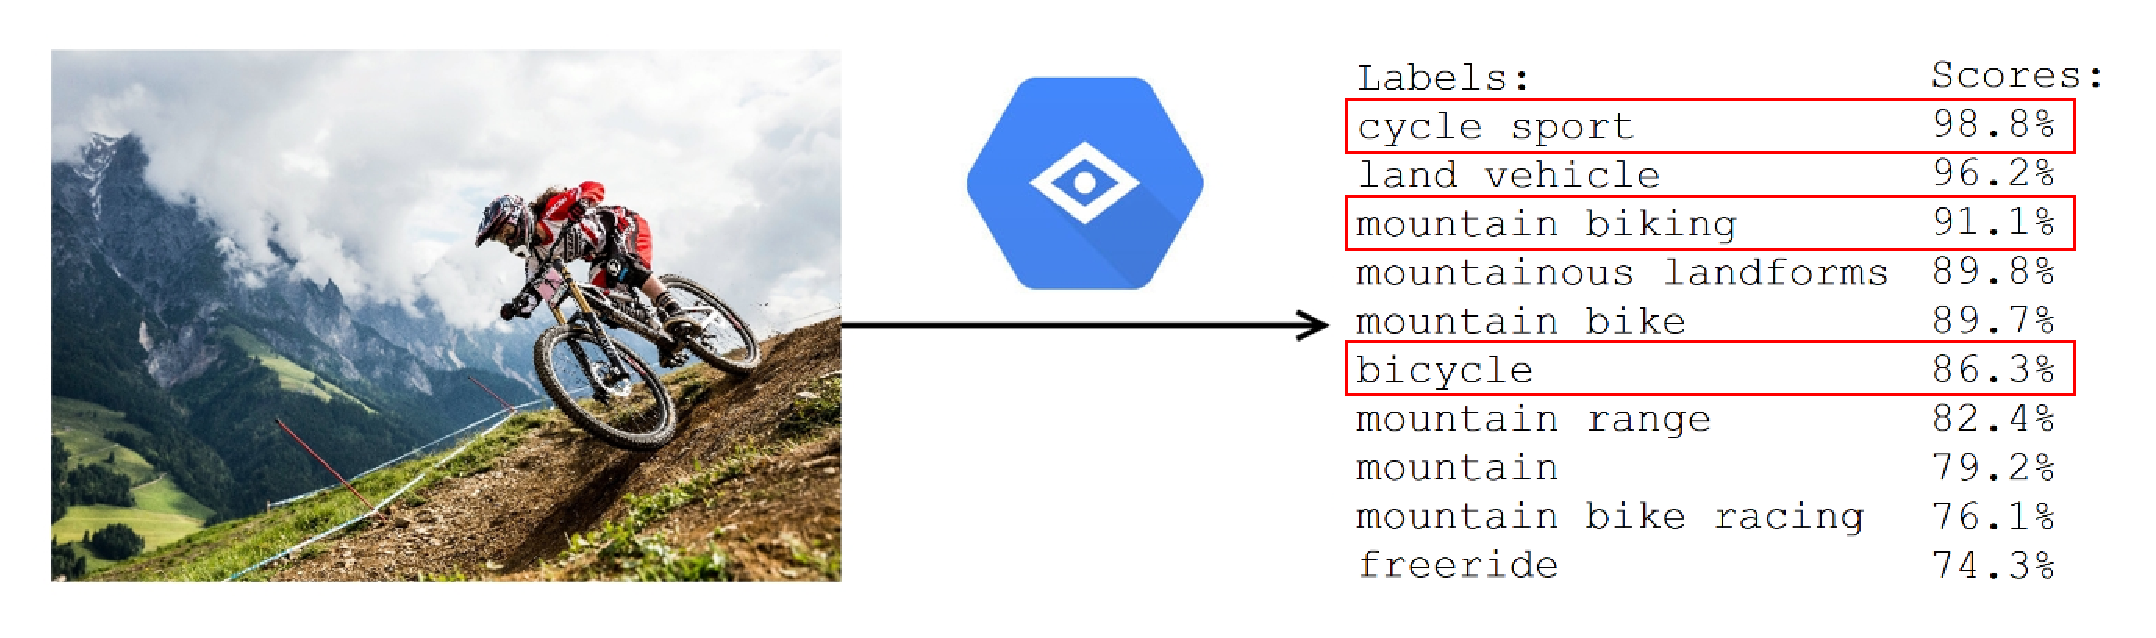
\includegraphics[width=0.75\textwidth]{img/vision_illustration.eps}
   \caption{This visualisation shall illustrate the image recognition process which is performed by the Google Cloud Vision API \parencite{2015ImageBiker}}
   \label{fig:vision_illustration}
\end{figure}

The placement of this entire step in relation to the other data- and text-processes is visualised in step 2 of figure \ref{XY}.

\subsection{Query costs} \label{vision_query_cost}
Google allows the creation of one Google Cloud trial account (needs a valid Credit Card for verification) per user which comes with 300 US Dollars’ worth of credit to one’s disposal. This credit can be used among others to rent virtual machines (VM’s), API’s and other Google Cloud services.\\
\newline
he Google Cloud Vision API can also be paid with that available credit and comes with the following rates: The first 1’000 requests per month are free of charge. The following requests up to 5 million requests per month are charged at \$1.50 per 1’000 requests – this applies specifically to the API specific label detection feature. Therefore, the 300\$ worth of credit would allow the processing of around 201’000 images \parencite{2019GooglePricing}. These rates were in place during the time of writing (January 2019) and will mostly likely vary with time.

\section{Machine Learning for text classification} 
\subsection{Background}
To understand how machine learning (ML) functions on text data, one first has to understand how it works on machine readable numerical data.\\
ML in its core refers to the process of a computer to understand or ‘learn’ the relationships inside a dataset with the help of algorithms to be able to make predictions on data the model has never seen before. The training's data normally consists of different features which identify and characterise a given entry. The constellation of feature-values which can be metaphorical seen as a ‘fingerprint’ of a given data point are the reason why a model can potentially make out patterns and relate them to a certain output. This output can either be a class (in the case of a classification problem) or a continuous number (in the case of a regression problem) of new data point.\\
\newline
One simple example of potential features could be different body-measurements of a specific animal with the aim to differentiate between different types of the same species. The training's data would then consist of multiple entries, where most likely a human measured all the needed body parts of several individuals and entered the numerical value in the corresponding feature field.\\

One can differentiate between two general types of ML – supervised and unsupervised learning. To illustrate the difference - imagine a set of training's data where each entry is represented by a point in an n-dimensional space where n corresponds to the number of features present and the coordinates of each point correspond to the feature’s values. If we make the link back to the example above, then unsupervised learning would mean that the training's data consists of only the training's data without any labels. The labels in this case would have been the names of the animal species that the measurements were taken from. In this way the model is forced to find natural breaks / boundaries on its own in the training data by clustering similar data points together and regarding them as an independent class. The hypothesis here is, that points closer to each other in space are more related / similar to one another than distant ones. This model given class name does not correspond in any way to the actual name of the animal, because the model has no information on it what so ever. It is up to the user to appropriately label the clusters / classes the model isolated.
Supervised learning on the other hand happens when the model is fed and trained upon example data with their correct classification labels present. The term ‘supervised’ therefore relates to the fact that presumably a human told the model which data points belong to which class. This approach is understandably more laborious because the creation of a labelled training-data set takes time, but it allows for a better performing model and its direct validation. Validation is done by splitting the original training-data set into two parts. Generally, a bigger portion is used for training the model and the other one - which the model has never seen during the fitting phase - is used to assess the model’s performance.\\
\newline
These terms correspond to two extremes of how the model and its incorporated (boundary-) function is fitted to the provided test-data (see point in figure \ref{XY}). Underfitting describes the state, where the model does not seem to extract and comprehend any logic from the dataset and therefore over-generalises the classification problem at hand (see outer left graph of figure \ref{fig:over_underfitting}). The other extreme is known by the term overfitting where the model tries to correctly classify every single training-data point to its proper class. This results in the model being extremely tuned to the provided training-data but not being able to generalise well on new, unseen data (see outer right graph in figure \ref{fig:over_underfitting}).\\
Underfitting is more easily detected and corrected than overfitting but more on that topic in chapter \ref{ml_text_data} Machine learning on non-numerical text data.

\begin{figure}[h]
   \centering
   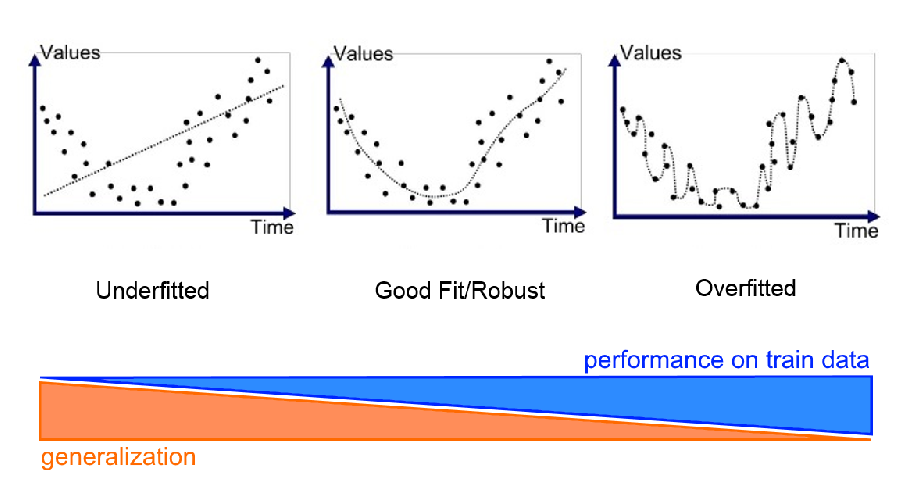
\includegraphics[width=0.75\textwidth]{img/over_underfitting.eps}
   \caption{Visualisation of under- and overfitting on a dataset. Altered image by author from\parencite{Bhande2018WhatIt.}}
   \label{fig:over_underfitting}
\end{figure}

\subsection{Machine learning on non-numerical text data} \label{ml_text_data}

One approach to transform text-based data into machine readable information will be covered in this chapter. Steps 3, 4, 5 and 6 of figure \ref{fig:ml_visualisation} to the left can be used as reference and will illustrate the described processes.\\
There are multiple approaches available to process text, but outputting numbers at the end in one form or the other is what they all have in common.\\
In this project the \textit{bag-of-words} representation has been applied \parencite{Joulin2016BagClassification}. This method learns the ‘vocabulary’ of a corpus of documents – in this case referred to as media objects. Then associates a sequence of numbers representing words present and missing from the corpus vocabulary to each individual media as a ‘fingerprint’. The entire process can be boiled down into three steps which explain more thoroughly what has been said above:

\paragraph{Tokenization} The input - consisting of the concatenated text strings and the image recognition labels - of each media object is processed into word tokens by a sequence of various functions as seen in chapter \ref{text_processing} ‘Text-processing’ and step 4 of figure \ref{fig:ml_visualisation}. This homogenisation enables a reduced model complexity by merging similar features and neglecting features with little semantic meaning. The generated string outputs (see \ref{fig:ml_visualisation} step 5) are fed into:

\paragraph{Vocabulary building} By assessing the individual word tokens of each media object, the ‘bag-of-words’ constructor assembles a vocabulary of unique tokens found in the corpus. This ‘vocabulary’ so to speak appears in the shape of an alphabetic ordered array where each column represents a word token. These columns are from now on referred to as a (model) features.

\paragraph{Encoding} The previously build vocabulary array is iterated through and compared to the word tokens found in the final text string of each media object for which a ‘fingerprint’-array is instantiated. Missing words are recorded as nulls and appearances are recorded by their count. This results in a number sequence linked to a given media object on which the model is later trained.

\begin{figure}[h]
   \centering
   \includegraphics[width=0.5\textwidth, left]{img/ML_text_data_visualization.eps}
   \caption{}
   \label{fig:ml_visualisation}
\end{figure}

\subsection{Recreation-types}










